% Generated by Sphinx.
\def\sphinxdocclass{report}
\documentclass[a4paper,10pt,english]{sphinxmanual}
\usepackage[utf8]{inputenc}
\DeclareUnicodeCharacter{00A0}{\nobreakspace}
\usepackage{cmap}
\usepackage[T1]{fontenc}
\usepackage{babel}
\usepackage{times}
\usepackage[Bjarne]{fncychap}
\usepackage{longtable}
\usepackage{sphinx}
\usepackage{multirow}

\usepackage{typo3}

\title{Datec Timeline}
\date{2016-02-22 17:48}
\release{1.1.0}
\author{Philipp Roensch}
\newcommand{\sphinxlogo}{}
\renewcommand{\releasename}{Release}
\makeindex

\makeatletter
\def\PYG@reset{\let\PYG@it=\relax \let\PYG@bf=\relax%
    \let\PYG@ul=\relax \let\PYG@tc=\relax%
    \let\PYG@bc=\relax \let\PYG@ff=\relax}
\def\PYG@tok#1{\csname PYG@tok@#1\endcsname}
\def\PYG@toks#1+{\ifx\relax#1\empty\else%
    \PYG@tok{#1}\expandafter\PYG@toks\fi}
\def\PYG@do#1{\PYG@bc{\PYG@tc{\PYG@ul{%
    \PYG@it{\PYG@bf{\PYG@ff{#1}}}}}}}
\def\PYG#1#2{\PYG@reset\PYG@toks#1+\relax+\PYG@do{#2}}

\expandafter\def\csname PYG@tok@ge\endcsname{\let\PYG@it=\textit}
\expandafter\def\csname PYG@tok@vg\endcsname{\def\PYG@tc##1{\textcolor[rgb]{0.73,0.38,0.84}{##1}}}
\expandafter\def\csname PYG@tok@ss\endcsname{\def\PYG@tc##1{\textcolor[rgb]{0.32,0.47,0.09}{##1}}}
\expandafter\def\csname PYG@tok@gp\endcsname{\let\PYG@bf=\textbf\def\PYG@tc##1{\textcolor[rgb]{0.78,0.36,0.04}{##1}}}
\expandafter\def\csname PYG@tok@mh\endcsname{\def\PYG@tc##1{\textcolor[rgb]{0.13,0.50,0.31}{##1}}}
\expandafter\def\csname PYG@tok@c\endcsname{\let\PYG@it=\textit\def\PYG@tc##1{\textcolor[rgb]{0.25,0.50,0.56}{##1}}}
\expandafter\def\csname PYG@tok@cp\endcsname{\def\PYG@tc##1{\textcolor[rgb]{0.00,0.44,0.13}{##1}}}
\expandafter\def\csname PYG@tok@kn\endcsname{\let\PYG@bf=\textbf\def\PYG@tc##1{\textcolor[rgb]{0.00,0.44,0.13}{##1}}}
\expandafter\def\csname PYG@tok@kt\endcsname{\def\PYG@tc##1{\textcolor[rgb]{0.56,0.13,0.00}{##1}}}
\expandafter\def\csname PYG@tok@nb\endcsname{\def\PYG@tc##1{\textcolor[rgb]{0.00,0.44,0.13}{##1}}}
\expandafter\def\csname PYG@tok@k\endcsname{\let\PYG@bf=\textbf\def\PYG@tc##1{\textcolor[rgb]{0.00,0.44,0.13}{##1}}}
\expandafter\def\csname PYG@tok@cm\endcsname{\let\PYG@it=\textit\def\PYG@tc##1{\textcolor[rgb]{0.25,0.50,0.56}{##1}}}
\expandafter\def\csname PYG@tok@gi\endcsname{\def\PYG@tc##1{\textcolor[rgb]{0.00,0.63,0.00}{##1}}}
\expandafter\def\csname PYG@tok@nc\endcsname{\let\PYG@bf=\textbf\def\PYG@tc##1{\textcolor[rgb]{0.05,0.52,0.71}{##1}}}
\expandafter\def\csname PYG@tok@nl\endcsname{\let\PYG@bf=\textbf\def\PYG@tc##1{\textcolor[rgb]{0.00,0.13,0.44}{##1}}}
\expandafter\def\csname PYG@tok@mi\endcsname{\def\PYG@tc##1{\textcolor[rgb]{0.13,0.50,0.31}{##1}}}
\expandafter\def\csname PYG@tok@sd\endcsname{\let\PYG@it=\textit\def\PYG@tc##1{\textcolor[rgb]{0.25,0.44,0.63}{##1}}}
\expandafter\def\csname PYG@tok@bp\endcsname{\def\PYG@tc##1{\textcolor[rgb]{0.00,0.44,0.13}{##1}}}
\expandafter\def\csname PYG@tok@il\endcsname{\def\PYG@tc##1{\textcolor[rgb]{0.13,0.50,0.31}{##1}}}
\expandafter\def\csname PYG@tok@s1\endcsname{\def\PYG@tc##1{\textcolor[rgb]{0.25,0.44,0.63}{##1}}}
\expandafter\def\csname PYG@tok@kp\endcsname{\def\PYG@tc##1{\textcolor[rgb]{0.00,0.44,0.13}{##1}}}
\expandafter\def\csname PYG@tok@gt\endcsname{\def\PYG@tc##1{\textcolor[rgb]{0.00,0.27,0.87}{##1}}}
\expandafter\def\csname PYG@tok@vc\endcsname{\def\PYG@tc##1{\textcolor[rgb]{0.73,0.38,0.84}{##1}}}
\expandafter\def\csname PYG@tok@s\endcsname{\def\PYG@tc##1{\textcolor[rgb]{0.25,0.44,0.63}{##1}}}
\expandafter\def\csname PYG@tok@vi\endcsname{\def\PYG@tc##1{\textcolor[rgb]{0.73,0.38,0.84}{##1}}}
\expandafter\def\csname PYG@tok@no\endcsname{\def\PYG@tc##1{\textcolor[rgb]{0.38,0.68,0.84}{##1}}}
\expandafter\def\csname PYG@tok@se\endcsname{\let\PYG@bf=\textbf\def\PYG@tc##1{\textcolor[rgb]{0.25,0.44,0.63}{##1}}}
\expandafter\def\csname PYG@tok@ni\endcsname{\let\PYG@bf=\textbf\def\PYG@tc##1{\textcolor[rgb]{0.84,0.33,0.22}{##1}}}
\expandafter\def\csname PYG@tok@ne\endcsname{\def\PYG@tc##1{\textcolor[rgb]{0.00,0.44,0.13}{##1}}}
\expandafter\def\csname PYG@tok@gh\endcsname{\let\PYG@bf=\textbf\def\PYG@tc##1{\textcolor[rgb]{0.00,0.00,0.50}{##1}}}
\expandafter\def\csname PYG@tok@nf\endcsname{\def\PYG@tc##1{\textcolor[rgb]{0.02,0.16,0.49}{##1}}}
\expandafter\def\csname PYG@tok@nd\endcsname{\let\PYG@bf=\textbf\def\PYG@tc##1{\textcolor[rgb]{0.33,0.33,0.33}{##1}}}
\expandafter\def\csname PYG@tok@mf\endcsname{\def\PYG@tc##1{\textcolor[rgb]{0.13,0.50,0.31}{##1}}}
\expandafter\def\csname PYG@tok@s2\endcsname{\def\PYG@tc##1{\textcolor[rgb]{0.25,0.44,0.63}{##1}}}
\expandafter\def\csname PYG@tok@sh\endcsname{\def\PYG@tc##1{\textcolor[rgb]{0.25,0.44,0.63}{##1}}}
\expandafter\def\csname PYG@tok@sb\endcsname{\def\PYG@tc##1{\textcolor[rgb]{0.25,0.44,0.63}{##1}}}
\expandafter\def\csname PYG@tok@o\endcsname{\def\PYG@tc##1{\textcolor[rgb]{0.40,0.40,0.40}{##1}}}
\expandafter\def\csname PYG@tok@w\endcsname{\def\PYG@tc##1{\textcolor[rgb]{0.73,0.73,0.73}{##1}}}
\expandafter\def\csname PYG@tok@sc\endcsname{\def\PYG@tc##1{\textcolor[rgb]{0.25,0.44,0.63}{##1}}}
\expandafter\def\csname PYG@tok@ow\endcsname{\let\PYG@bf=\textbf\def\PYG@tc##1{\textcolor[rgb]{0.00,0.44,0.13}{##1}}}
\expandafter\def\csname PYG@tok@go\endcsname{\def\PYG@tc##1{\textcolor[rgb]{0.20,0.20,0.20}{##1}}}
\expandafter\def\csname PYG@tok@sr\endcsname{\def\PYG@tc##1{\textcolor[rgb]{0.14,0.33,0.53}{##1}}}
\expandafter\def\csname PYG@tok@si\endcsname{\let\PYG@it=\textit\def\PYG@tc##1{\textcolor[rgb]{0.44,0.63,0.82}{##1}}}
\expandafter\def\csname PYG@tok@mb\endcsname{\def\PYG@tc##1{\textcolor[rgb]{0.13,0.50,0.31}{##1}}}
\expandafter\def\csname PYG@tok@nn\endcsname{\let\PYG@bf=\textbf\def\PYG@tc##1{\textcolor[rgb]{0.05,0.52,0.71}{##1}}}
\expandafter\def\csname PYG@tok@kd\endcsname{\let\PYG@bf=\textbf\def\PYG@tc##1{\textcolor[rgb]{0.00,0.44,0.13}{##1}}}
\expandafter\def\csname PYG@tok@sx\endcsname{\def\PYG@tc##1{\textcolor[rgb]{0.78,0.36,0.04}{##1}}}
\expandafter\def\csname PYG@tok@m\endcsname{\def\PYG@tc##1{\textcolor[rgb]{0.13,0.50,0.31}{##1}}}
\expandafter\def\csname PYG@tok@gr\endcsname{\def\PYG@tc##1{\textcolor[rgb]{1.00,0.00,0.00}{##1}}}
\expandafter\def\csname PYG@tok@mo\endcsname{\def\PYG@tc##1{\textcolor[rgb]{0.13,0.50,0.31}{##1}}}
\expandafter\def\csname PYG@tok@cs\endcsname{\def\PYG@tc##1{\textcolor[rgb]{0.25,0.50,0.56}{##1}}\def\PYG@bc##1{\setlength{\fboxsep}{0pt}\colorbox[rgb]{1.00,0.94,0.94}{\strut ##1}}}
\expandafter\def\csname PYG@tok@kc\endcsname{\let\PYG@bf=\textbf\def\PYG@tc##1{\textcolor[rgb]{0.00,0.44,0.13}{##1}}}
\expandafter\def\csname PYG@tok@c1\endcsname{\let\PYG@it=\textit\def\PYG@tc##1{\textcolor[rgb]{0.25,0.50,0.56}{##1}}}
\expandafter\def\csname PYG@tok@na\endcsname{\def\PYG@tc##1{\textcolor[rgb]{0.25,0.44,0.63}{##1}}}
\expandafter\def\csname PYG@tok@err\endcsname{\def\PYG@bc##1{\setlength{\fboxsep}{0pt}\fcolorbox[rgb]{1.00,0.00,0.00}{1,1,1}{\strut ##1}}}
\expandafter\def\csname PYG@tok@gs\endcsname{\let\PYG@bf=\textbf}
\expandafter\def\csname PYG@tok@gd\endcsname{\def\PYG@tc##1{\textcolor[rgb]{0.63,0.00,0.00}{##1}}}
\expandafter\def\csname PYG@tok@nv\endcsname{\def\PYG@tc##1{\textcolor[rgb]{0.73,0.38,0.84}{##1}}}
\expandafter\def\csname PYG@tok@kr\endcsname{\let\PYG@bf=\textbf\def\PYG@tc##1{\textcolor[rgb]{0.00,0.44,0.13}{##1}}}
\expandafter\def\csname PYG@tok@nt\endcsname{\let\PYG@bf=\textbf\def\PYG@tc##1{\textcolor[rgb]{0.02,0.16,0.45}{##1}}}
\expandafter\def\csname PYG@tok@gu\endcsname{\let\PYG@bf=\textbf\def\PYG@tc##1{\textcolor[rgb]{0.50,0.00,0.50}{##1}}}

\def\PYGZbs{\char`\\}
\def\PYGZus{\char`\_}
\def\PYGZob{\char`\{}
\def\PYGZcb{\char`\}}
\def\PYGZca{\char`\^}
\def\PYGZam{\char`\&}
\def\PYGZlt{\char`\<}
\def\PYGZgt{\char`\>}
\def\PYGZsh{\char`\#}
\def\PYGZpc{\char`\%}
\def\PYGZdl{\char`\$}
\def\PYGZhy{\char`\-}
\def\PYGZsq{\char`\'}
\def\PYGZdq{\char`\"}
\def\PYGZti{\char`\~}
% for compatibility with earlier versions
\def\PYGZat{@}
\def\PYGZlb{[}
\def\PYGZrb{]}
\makeatother

\renewcommand\PYGZsq{\textquotesingle}

\begin{document}

\maketitle
\tableofcontents
\phantomsection\label{Index::doc}



\chapter{What does it do?}
\label{Introduction/Index:start}\label{Introduction/Index:datec-timeline}\label{Introduction/Index::doc}\label{Introduction/Index:what-does-it-do}\label{Introduction/Index:introduction}
This extension gives a basic appointment model to organize appointments. The frontend solution is jQuery FullCalendar, which requires jQuery and jQuery-ui to be installed.
The extension frontend is based on fullcalendar functionality, combined with the appointment object, perfect to handle appointmens with multiple participants:
\begin{itemize}
\item {} 
Calendar and agenda views per month, week or day

\item {} 
Appointments can be edited in frontend view, dragging and moving events is supported

\item {} 
Appointments have title, description, creator or participants assigned from frontent users and a reminder date

\item {} 
Access to the plugins features can be controlled with access rights to the plugin content element

\item {} 
Frontend view is optimized for responsive design and testet with Bootstrap 3

\end{itemize}

\begin{notice}{tip}{Tip:}
Visit \& contribute: \href{https://github.com/theorak/datec\_timeline}{https://github.com/theorak/datec\_timeline}
\end{notice}

\begin{notice}{tip}{Tip:}
More information about fullcalendar: \href{http://fullcalendar.io/}{http://fullcalendar.io/}
\end{notice}
\begin{figure}[htbp]
\centering
\capstart

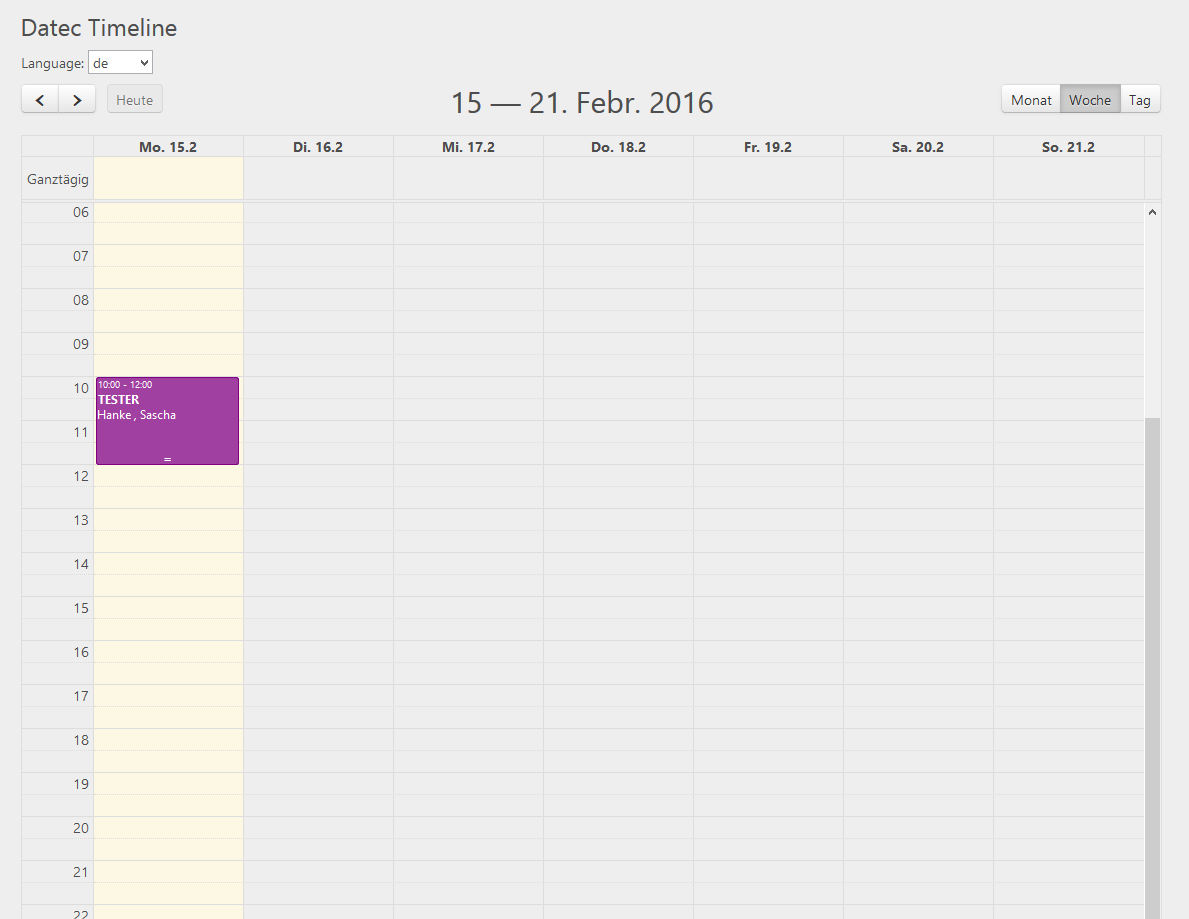
\includegraphics{datec_timeline_01_overview.png}
\caption{Datec Timeline just after installation}\end{figure}


\chapter{Users manual}
\label{UsersManual/Index:id1}\label{UsersManual/Index:users-manual}\label{UsersManual/Index::doc}
Target group: \textbf{Users and Editors}


\section{Editors - Creator of Appointments}
\label{UsersManual/Index:editors-creator-of-appointments}
The color that appointments appear in is based around the creator of that appointment. All creators are frontend users, thus to change his color, look for the Date Color option in the users data.
\begin{figure}[htbp]
\centering
\capstart

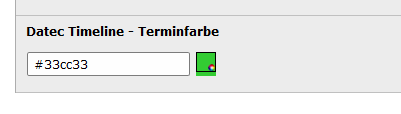
\includegraphics{datec_timeline_04_creator1.png}
\caption{Editing Frontend users as creators}\end{figure}


\section{Users - Views}
\label{UsersManual/Index:users-views}
The default view is fullcalendar's ``Agenda Week'' view. This view is optimal for appointments with time information.
The controls on the right also let the user switch between monthly and per day view, the latter is forced as default for mobilde devices or small screens.
Also above the timeline you'll find the list of creators of appointments, click them to filter the viewed appointments.
This view will refresh every 30 seconds.
\begin{figure}[htbp]
\centering
\capstart

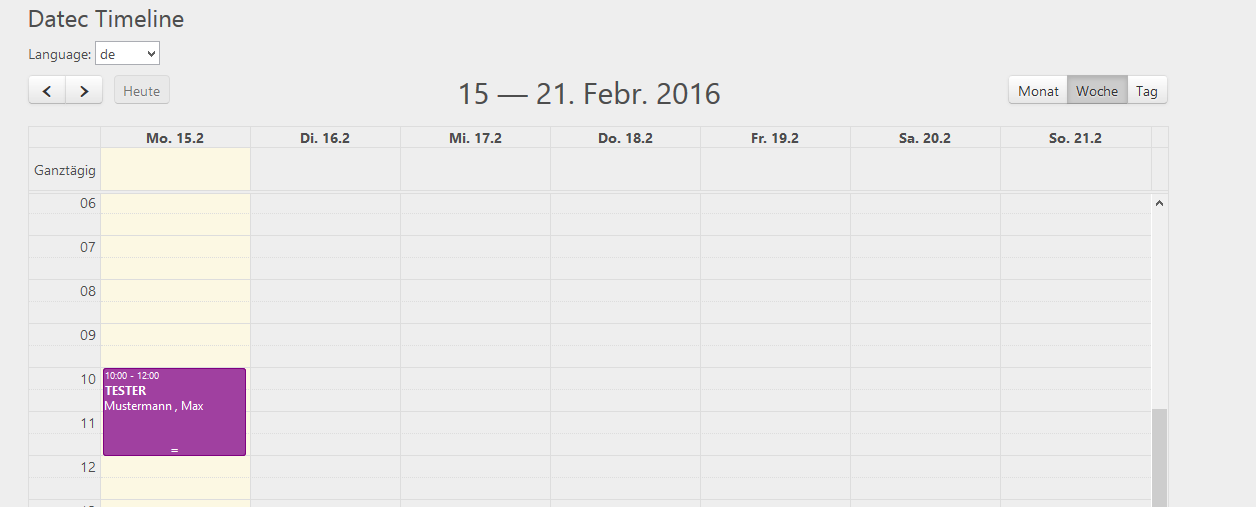
\includegraphics{datec_timeline_02_views1.png}
\caption{Viewing of appointmets}\end{figure}


\section{Users - Creating and Editing}
\label{UsersManual/Index:users-creating-and-editing}
Users can create and edit appointments right in the frontend. Just click on any spot in the timeline and a popup window for all necessary properties appears:
- Title: the title of the appointment.
- Description: A short description of the appointment.
- Participants: A list of other frontend-users to invite to this appointment.
- From/To: The date-time range of the appointment, prefilled with the selected date.
- Reminder From: Automatic reminder e-mails will be send after this date, prefilled with the start of the appointment.
Note: The currently logged in frontend user is saved as the creator of the appointment.

The appointment can then be edited again, by simply clicking on it, or moving it to a desired date.
\begin{figure}[htbp]
\centering
\capstart

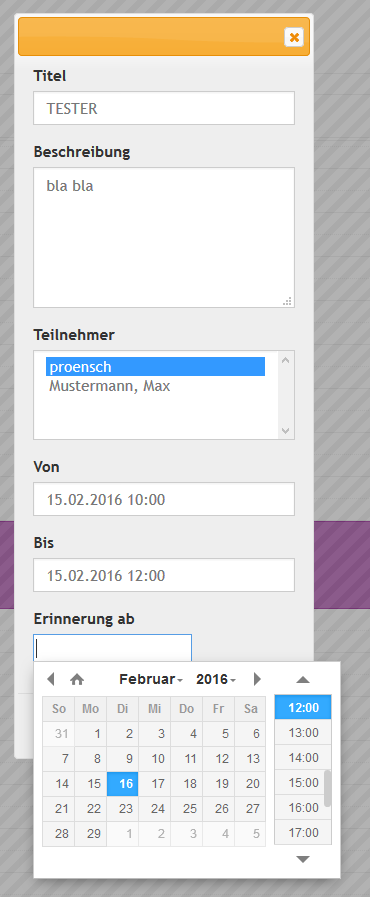
\includegraphics{datec_timeline_03_createdate1.png}
\caption{Viewing of appointmets}\end{figure}


\chapter{Administrator Manual}
\label{AdministratorManual/Index::doc}\label{AdministratorManual/Index:admin-manual}\label{AdministratorManual/Index:administrator-manual}
Target group: \textbf{Administrators}


\section{Requirements}
\label{AdministratorManual/Index:requirements}
\begin{notice}{caution}{Caution:}
You must load the jQuery JavaScript framework ans jQuery-uid plugin yourself as the frontend plugin utilizes functions that depend on these libraries.
\end{notice}


\section{Installation}
\label{AdministratorManual/Index:installation}\begin{enumerate}
\item {} 
Download and install the extension via the extension manager (extKey: datec\_timeline).

\item {} 
Add one storage folder for appointments, note down the page id (PID) of this folder.

\item {} 
Check the Configuration section of this manual for the required configuration and follow the steps there.

\item {} 
Insert the main plugin as described below.

\item {} 
(optional) Add the scheduler task for appointment reminder e-mails.

\end{enumerate}


\section{Insert Plugin}
\label{AdministratorManual/Index:insert-plugin}\begin{enumerate}
\item {} 
Insert a content element, choose ``Plugins'' -\textgreater{} ``General Plugin''

\end{enumerate}
\begin{figure}[htbp]
\centering
\capstart

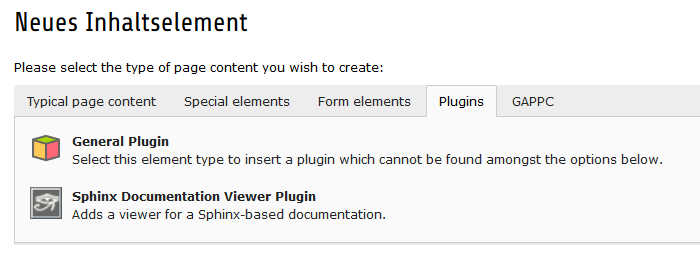
\includegraphics{plugin_01.png}
\caption{Inserting content element of type ``Plugin''}\end{figure}
\begin{enumerate}
\setcounter{enumi}{1}
\item {} 
Choose the plugin ``Datec Timeline''.

\end{enumerate}
\begin{figure}[htbp]
\centering
\capstart

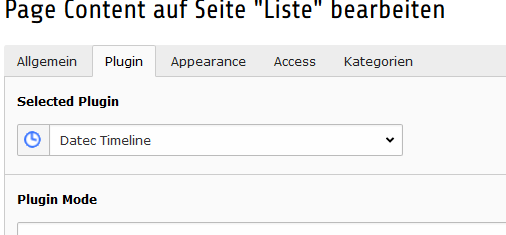
\includegraphics{plugin_02.png}
\caption{Choosing a display form}\end{figure}
\begin{enumerate}
\setcounter{enumi}{2}
\item {} 
(optional) Set access rights as required, appointments should have a closed group of users.

\end{enumerate}


\section{Add Reminder E-mail Task}
\label{AdministratorManual/Index:add-reminder-e-mail-task}\begin{enumerate}
\item {} 
Goto the BE-Mudole scheduler (scheduler extension must be installed and configured).

\item {} 
Add a new scheduler task ``Datec Timeline - Reminder e-mails task''

\item {} 
It is recommended to set a recurring, daily task (86400 seconds) and set the time of execution time to 0:00 am.

\item {} 
Note that the e-mail language depends on the langue setting of the \_cli\_scheduler backend user.

\end{enumerate}

Target group: \textbf{Administrators}


\chapter{Configuration Reference}
\label{Configuration/Index:configuration}\label{Configuration/Index::doc}\label{Configuration/Index:configuration-reference}
This section describes all options aviable for Datec Timeline via TypoScript setup. To change these options please add a new extension template to your ROOT template.


\section{Minimal configuration}
\label{Configuration/Index:configuration-typoscript}\label{Configuration/Index:minimal-configuration}
Upon installation, please add the static extension template `Datec Timeline' to your ROOT template (Web \textgreater{} Template \textgreater{} edit root page template \textgreater{} Includes \textgreater{} select static template from extensions) and set at least the following options:

\begin{Verbatim}[frame=single,commandchars=\\\{\}]
\PYGZsh{} PID of your storage folder for appointments
plugin.tx\PYGZus{}datectimeline.persistence.storagePid = 123
plugin.tx\PYGZus{}datectimeline.settings.storagePid = 123

\PYGZsh{} Valid e\PYGZhy{}mail address to dispatch automatic mails from
plugin.tx\PYGZus{}datectimeline.settings.mail.internMailFrom = timeline@no\PYGZhy{}reply.com
\end{Verbatim}


\section{General configuration}
\label{Configuration/Index:general-configuration}
plugin.tx\_datectimeline.

\begin{tabulary}{\linewidth}{|L|L|L|L|}
\hline
\textsf{\relax 
Property
} & \textsf{\relax 
Data type
} & \textsf{\relax 
Description
} & \textsf{\relax 
Default
}\\
\hline
view.templateRootPaths
 & 
array
 & 
Constant, path to template files if you wish to use your own.
 & 
EXT:datec\_timeline/Resources/Private/Templates/
\\
\hline
view.partialRootPaths
 & 
array
 & 
Constant, path to partial template files if you wish to use your own.
 & 
EXT:datec\_timeline/Resources/Private/Partials/
\\
\hline
view.layoutRootPaths
 & 
array
 & 
Constant, path to layout files if you wish to use your own.
 & 
EXT:datec\_timeline/Resources/Private/Layouts/
\\
\hline
persistence.storagePid
 & 
int
 & 
System folder for appointments.
 & \\
\hline
settings.storagePid
 & 
int
 & 
System folder for appointments.
 & \\
\hline
settings.mail.internMailFrom
 & 
string
 & 
E-mail address for automatic notification Mails {[}FROM{]}.
 & 
\href{mailto:timeline@no-reply.com}{timeline@no-reply.com}
\\
\hline
settings.mail.internMailFromName
 & 
string
 & 
Name to display for automatic notification Mails {[}FROM-NAME{]}.
 & 
Datec Timeline
\\
\hline
settings.display.comments.dateFormat
 & 
string
 & 
Like `settings.display.dateFormat' for comments only.
 & 
d.m.Y - H:
\\
\hline
settings.reminderMailAfterCreation
 & 
string
 & 
Send out first reminder E-Mail after creation of appointment.
 & 
true
\\
\hline
settings.reminderMailAfterEdit
 & 
string
 & 
Send out a reminder E-Mail after each edit of appointment.
 & 
true
\\
\hline
settings.langOptions
 & 
string
 & 
Hides/shows language options.
 & 
true
\\
\hline\end{tabulary}



\chapter{Known Problems}
\label{KnownProblems/Index:id1}\label{KnownProblems/Index:known-problems}\label{KnownProblems/Index::doc}
No problems reported yet.

Issues will be tracked \href{https://github.com/theorak/datec\_timeline}{here}


\chapter{To-Do List}
\label{ToDoList/Index:id1}\label{ToDoList/Index:to-do-list}\label{ToDoList/Index::doc}
All is well.

See current development \href{https://github.com/theorak/datec\_timeline}{here}


\chapter{Change Log}
\label{ChangeLog/Index:id1}\label{ChangeLog/Index::doc}\label{ChangeLog/Index:change-log}
Changes will be tracked \href{https://github.com/theorak/datec\_timeline}{here}.


\chapter{FAQ}
\label{FAQ/Index:id1}\label{FAQ/Index::doc}\label{FAQ/Index:faq}

\section{How to change the layout/design?}
\label{FAQ/Index:how-to-change-the-layout-design}
Copy the template files (\code{datec\_timeline\textbackslash{}Resources\textbackslash{}Private\textbackslash{}Layouts} \textbackslash{}Partials, \textbackslash{}Templates)
into the fileadmin folder and change the paths via TS or constant editor (see the configuration section of this document).



\renewcommand{\indexname}{Index}
\printindex
\end{document}
